%-------------------------------------------------------------------------
% fonctions-2.tex
%-------------------------------------------------------------------------

%-------------------------------------------------------------------------
\setjobnamebeamerversion{fonctions-2Slide}

\usetheme{Enib}
%-------------------------------------------------------------------------

%-------------------------------------------------------------------------
\newtheorem{rem}{Remarque}[section]
\newtheorem{defin}{Définition}[section]
\newtheorem{td}{\color{blue}TD}[section]
%-------------------------------------------------------------------------

%-------------------------------------------------------------------------
\lstset
{
language=Python,
basicstyle=\ttfamily,
identifierstyle=\ttfamily,
keywordstyle=\color{blue}\ttfamily,
commentstyle=\color{gray}\ttfamily,
stringstyle=\color{green}\ttfamily,
showstringspaces=false,
extendedchars=true,
numbers=left, 
numberstyle=\tiny,
frame=lines,
linewidth=0.95\textwidth,
xleftmargin=5mm
} 
%-------------------------------------------------------------------------

%-------------------------------------------------------------------------
\def\exo#1{\mbox{}\ \hfill\mbox{\color{blue}$\rule{2mm}{2mm}\,$\footnotesize\sc TD\ref{#1}}}
\def\exercice#1#2{\mbox{}\ \ TD \ref{#1}\ #2\ \dotfill\ \pageref{#1}\mbox{}}

\newenvironment{py}[1]{\begin{minipage}[t]{#1}\footnotesize}{\end{minipage}}
%-------------------------------------------------------------------------

\graphicspath{{../../fig/}}

%-------------------------------------------------------------------------
\title[Algorithmique]{\bf Initiation à l'algorithmique}
\subtitle{\bf --- procédures et fonctions ---\newline
2. Appel d'une fonction}

\author[\tt jacques.tisseau@enib.fr]{\large\bf Jacques TISSEAU}
\institute[\enib]{{\large\enib--\cerv}}
\date[enib\copyright 2009-2014]{\footnotesize enib\copyright 2009-2014}
%-------------------------------------------------------------------------

%-------------------------------------------------------------------------
\begin{document}
%-------------------------------------------------------------------------

%------------------------------------------
\begin{frame}
\frametitle{\uppercase{Informatique \hfill {S1}}}
%------------------------------------------
\titlepage

\end{frame}
\note{
\mbox{}\null\vfill

\begin{rem}[Notes de cours : couverture]
Ce support de cours accompagne le 
chapitre 3 des notes de cours « Initiation à l'algorithmique ».
$$\fbox{\includegraphics[width=10cm,page=1]{../../../pdf/cours/info-S1.pdf}}$$
\end{rem}
}
%------------------------------------------

%------------------------------------------
\begin{frame}[containsverbatim]
\frametitle{\uppercase{Appel de fonction}}
\framesubtitle{\uppercase{Fonction de Fibonacci}}
%------------------------------------------
\footnotesize
\begin{lstlisting}
def fibonacci(n):
    """ 
    u = fibonacci(n) 
    est le nombre de Fibonacci 
    a l'ordre n si n:int >= 0 
    """
    assert type(n) is int
    assert n >= 0
    u, u1, u2 = 1, 1, 1
    for i in range(2,n+1):
        u = u1 + u2
        u2 = u1
        u1 = u
    return u
\end{lstlisting}

\end{frame}
\note{
\begin{rem}[Fonction de Fibonacci]
La fonction de Fibonacci calcule le nombre $u_n$ à l'ordre $n$ (dit de Fibonacci) 
selon la relation de récurrence :
$$u_0 = 1\ ,\ u_1 = 1\ ,\ u_n = u_{n-1} + u_{n-2}\ \forall n \in N,\ n > 1$$
Les 10 premiers nombres de Fibonacci valent donc : $u_0 = 1$, $u_1 = 1$, $u_2 = 2$,
$u_3 = 3$, $u_4 = 5$, $u_5 = 8$, $u_6 = 13$, $u_7 = 21$, $u_8 = 34$ et $u_9 = 55$.

La suite de Fibonacci doit son nom au mathématicien italien Fibonacci (1175-1250). 
Dans un problème récréatif, Fibonacci décrit la croissance d'une population « idéale »
de lapins de la manière suivante :
\begin{itemize}
\item le premier mois, il y a juste une paire de lapereaux ;
\item les lapereaux ne sont pubères qu'à partir du deuxième mois ;
\item chaque mois, tout couple susceptible de procréer engendre effectivement 
	un nouveau couple de lapereaux ;
\item les lapins ne meurent jamais !
\end{itemize}
Se pose alors le problème suivant :
\begin{quote}\em
« Possédant initialement un couple de lapins, combien de couples obtient-on 
en douze mois si chaque couple engendre tous les mois un nouveau couple 
à compter du second mois de son existence ? »
\end{quote}
\end{rem}
}
%------------------------------------------

%------------------------------------------
\begin{frame}
\frametitle{\uppercase{Appel de fonction}}
\framesubtitle{\uppercase{Passage des paramètres}}
%------------------------------------------
%\centerline{\multiinclude[graphics={width=10cm},format=pdf]{param}}
\centerline{\includegraphics[width=10cm]{param-2.pdf}}
%\pause
\begin{description}
\item[à l'appel :] copie des paramètres effectifs dans les paramètres formels\\(\alert{\tt n = x})
%\pause
\item[à la sortie :] copie des paramètres formels dans les paramètres effectifs\\(\alert{\tt y = u})
%\pause
\vspace*{3mm}

\item[Passage par valeur :] ce ne sont pas les paramètres effectifs qui sont manipulés par la fonction mais des copies de ces paramètres
\end{description}
\end{frame}
\note{
{\bf Définitions}\begin{description}
\item[paramètre formel] paramètre d'entrée d'une fonction
	utilisé à l'in\-té\-rieur de la fonction appelée.
\item[paramètre effectif] paramètre d'appel d'une fonction
	utilisé à l'ex\-té\-rieur de la fonction appelée.
\item[passage par valeur] action de copier la valeur
	du paramètre effectif dans le paramètre formel
	correspondant.
\item[passage par référence] action de copier la référence
	du paramètre effectif dans le paramètre formel
	correspondant.
\end{description}
}
%------------------------------------------

%------------------------------------------
\begin{frame}
\frametitle{\uppercase{Appel de fonction}}
\framesubtitle{\uppercase{Appel équivalent}}
%------------------------------------------
\begin{columns}[T]
\column{5.25cm}
$$\begin{py}{5cm}
{\bf Appel :}\\\tt
%\begin{verbatim}
>{>}> x = 9\\
{\color{red}
>{>}> y = fibonacci(x)}\\
>{>}> y\\
55
\end{py}$$

%\pause
\column{5.25cm}
$$\begin{py}{5cm}
{\bf Appel équivalent :}\\\tt
>{>}> x = 9\\
%\pause
{\color{red} >{>}> n = x}\\
%\pause
{\color{blue}
>{>}> u, u1, u2 = 1, 1, 1\\
>{>}> for i in range(2,n+1):\\
... \ \ \ \ u = u1 + u2\\
... \ \ \ \ u2 = u1\\
... \ \ \ \ u1 = u\\
...}\\
%\pause
{\color{red} >{>}> tmp = u\\
%\pause
>{>}> del n, u, u1, u2, i\\
%\pause
>{>}> y = tmp\\
%\pause
>{>}> del tmp}\\
%\pause
>{>}> y\\
55
\end{py}$$
\end{columns}

\end{frame}
\note{
\null\vfill

\begin{td}[Passage par valeur]
On considère les codes suivants :

{\tt \mbox{}\ }\begin{py}{2.25cm}\tt
>{>}> x, y\\
(1, 2)\\
>{>}> tmp = x\\
>{>}> x = y\\
>{>}> y = tmp\\
>{>}> x, y\\
(2, 1)
\end{py}
\hfill
\begin{py}{3cm}\tt
def swap(x,y):\\
\mbox{}\ \ \ \ tmp = x\\
\mbox{}\ \ \ \ x = y\\
\mbox{}\ \ \ \ y = tmp\\
\mbox{}\ \ \ \ return
\end{py}
\hfill
\begin{py}{2.25cm}\tt
>{>}> x, y\\
(1, 2)\\
>{>}> swap(x,y)\\
>{>}> x, y\\
(1, 2)
\end{py}\\[1mm]
Expliquer la différence entre l'exécution de gauche et l'exécution de droite
en explicitant l'appel équivalent à l'appel {\tt swap(x,y)} dans l'exécution
de droite.
\end{td}
}
%------------------------------------------




%------------------------------------------
\begin{frame}
\frametitle{\uppercase{Appel de fonction}}
\framesubtitle{\uppercase{Portée des variables}}
%------------------------------------------
\centerline{\begin{py}{7.5cm}\tt
def f(x):\\
\mbox{}\ \ \ \ y = 3\\
\mbox{}\ \ \ \ x = x + y\\
\mbox{}\ \ \ \ print('liste :', dir())\\
\mbox{}\ \ \ \ print('intérieur :', locals())\\
\mbox{}\ \ \ \ print('extérieur :', globals())\\
\mbox{}\ \ \ \ return x\\
\end{py}}
%\pause


\centerline{\begin{py}{7.5cm}\tt
\alert{>{>}> y = 6\\
>{>}> f(6)}\\
%\pause
liste : ['x', 'y']\\%\pause
intérieur : \{'y': 3, 'x': 9\}\\%\pause
extérieur : \{'f': <function f at 0x822841c>,\\
\mbox{}\ \ \ \ \ \ \ \ \ \ \ \ \ 'y': 6,\\ 
\mbox{}\ \ \ \ \ \ \ \ \ \ \ \ \ '\_\_name\_\_': '\_\_main\_\_',\\
\mbox{}\ \ \ \ \ \ \ \ \ \ \ \ \ '\_\_doc\_\_': None\}\\
%\pause
\alert{9}
\end{py}}

\end{frame}
\note{
\null\vfill

\begin{td}[Portée des variables]
On considère les fonctions {\tt f}, {\tt g} et {\tt h} suivantes :

\begin{py}{2.5cm}\tt
def f(x):\\
\mbox{}\ \ x = 2*x\\
\mbox{}\ \ print('f', x)\\
\mbox{}\ \ return x
\end{py}
\hfill
\begin{py}{2.5cm}\tt
def g(x):\\
\mbox{}\ \ x = 2*f(x)\\
\mbox{}\ \ print('g', x)\\
\mbox{}\ \ return x
\end{py}
\hfill
\begin{py}{2.5cm}\tt
def h(x):\\
\mbox{}\ \ x = 2*g(f(x))\\
\mbox{}\ \ print('h', x)\\
\mbox{}\ \ return x
\end{py}
\mbox{}\vspace*{2mm}

Qu'affichent les appels suivants ?\\
\mbox{}\\
\begin{minipage}{3.5cm}
\begin{enumerate}
\item 
\begin{py}{2.5cm}\tt
>{>}> x = 5\\
>{>}> print(x)\\
{\color{red} ?}\\
>{>}> y = f(x)\\
>{>}> print(x)\\
{\color{red} ?}\\
>{>}> z = g(x)\\
>{>}> print(x)\\
{\color{red} ?}\\
>{>}> t = h(x)\\
>{>}> print(x)\\
{\color{red} ?}
\end{py}
\end{enumerate}
\end{minipage}
\hfill
\begin{minipage}{3.5cm}
\begin{enumerate}\setcounter{enumi}{1}
\item 
\begin{py}{2.5cm}\tt
>{>}> x = 5\\
>{>}> print(x)\\
{\color{red} ?}\\
>{>}> x = f(x)\\
>{>}> print(x)\\
{\color{red} ?}\\
>{>}> x = g(x)\\
>{>}> print(x)\\
{\color{red} ?}\\
>{>}> x = h(x)\\
>{>}> print(x)\\
{\color{red} ?}
\end{py}
\end{enumerate}
\end{minipage}
\end{td}
}
%------------------------------------------


%------------------------------------------
\begin{frame}
\frametitle{\uppercase{Appels récursifs}}
\framesubtitle{\uppercase{Fonction de Fibonacci}}
%------------------------------------------
$$u_0 = 1\ ,\ u_1 = 1\ ,\ u_n = u_{n-1} + u_{n-2}\ \forall n \in N,\ n > 1$$
%\pause
\begin{columns}[T]
\column{5.25cm}
\begin{py}{5.25cm}
{\bf Version itérative :}\\\tt
def fibonacci(n):\\
\mbox{}\ \ \ \ u, u1, u2 = 1, 1, 1\\
\mbox{}\ \ \ \ for i in range(2,n+1):\\
\mbox{}\ \ \ \ \ \ \ \ u = u1 + u2\\
\mbox{}\ \ \ \ \ \ \ \ u2 = u1\\
\mbox{}\ \ \ \ \ \ \ \ u1 = u\\
\mbox{}\ \ \ \ return u
\end{py}
%\pause

\column{5.25cm}
\begin{py}{5.25cm}
{\bf Version récursive :}\\\tt
def fibonacci(n):\\
\mbox{}\ \ \ \ u = 1\\
\mbox{}\ \ \ \ if n > 1:\\
\mbox{}\ \ \ \ \ \ \ \ \alert{u = fibonacci(n-1) + \\
\mbox{}\ \ \ \ \ \ \ \ \ \ \ \ fibonacci(n-2)}\\
\mbox{}\ \ \ \ return u
\end{py}
\end{columns}

\end{frame}
\note{
\null\vfill

\begin{td}[Puissance entière]
Définir une fonction récursive qui calcule la puissance entière $p = x^n$ 
d'un nombre entier $x$.
\end{td}

\begin{td}[Coefficients du binôme]
Définir une fonction récursive qui calcule les coefficients du binôme 
$\displaystyle (a+b)^n = \sum_{k=0}^n \frac{n!}{k!(n-k)!}a^{n-k}b^k$.
\end{td}

\begin{td}[Fonction d'Ackerman]
Définir une fonction récursive qui calcule la fonction d'Ackerman : 
$$
{f : N^2 \rightarrow N}\ 
\left\{\begin{array}{lll}
f{(0,n)} & = & n+1\\
f{(m,0)} & = & f{(m-1,1)}\mbox{\ si\ } m > 0\\
f{(m,n)} & = & f{(m-1,f{(m,n-1)})}\mbox{\ si\ } m > 0, n > 0
\end{array}\right.
$$
\end{td}
}
%------------------------------------------

%------------------------------------------
\begin{frame}
\frametitle{\uppercase{Appels récursifs}}
\framesubtitle{\uppercase{Fonction de Fibonacci}}
%------------------------------------------
\begin{columns}
\column{4cm}
\begin{minipage}{3.75cm}\tt
>{>}> fibonacci(5)\\
8
\end{minipage}
%\pause

\column{7cm}
$$\includegraphics[width=5cm]{recursivite.pdf}$$

\end{columns}

\end{frame}
\note{
\null\vfill

\begin{rem}[Récursivité en arbre : {\tt fibonacci}]
Dans la version récursive, pour calculer {\tt fibonacci(5)},
on calcule d'abord {\tt fibonac\-ci(4)} et {\tt fibonac\-ci(3)}. Pour calculer {\tt fibonacci(4)},
on calcule {\tt fibonac\-ci(3)} et {\tt fibonac\-ci(2)}.
Pour calculer {\tt fibonacci(3)}, on calcule {\tt fibonacci(2)} et {\tt fibonac\-ci(1)}\ldots\ 
Le dérou\-le\-ment du processus ressemble ainsi à un arbre  

On remarque 
que les branches de l'arbre se divise en deux à chaque niveau 
(sauf en bas de l'arbre, {\em ie} à droite sur la figure), 
ce qui traduit le fait que la fonction {\tt fibonacci} s'appelle elle-même deux fois 
à chaque fois qu'elle est invoquée avec {\tt n > 1}. 

Le nombre de feuilles dans l'arbre est précisément 
$u_n$ ({\tt fibonacci(n)}).
Or la valeur de $u_n$ croît de manière exponentielle avec $n$; ainsi, avec cette version récursive, 
le processus de calcul de {\tt fibonacci(n)} prend un temps qui croît de façon exponentielle
avec {\tt n}.
\end{rem}
}
%------------------------------------------

%------------------------------------------
\begin{frame}
\frametitle{\uppercase{Appels récursifs}}
\framesubtitle{\uppercase{Tours de Hanoï}}
%------------------------------------------
{\bf Etat initial :}\\[3mm]
\centerline{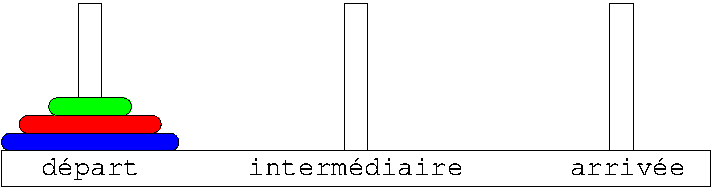
\includegraphics[width=8cm]{hanoi.pdf}}
\vspace*{1cm}

%\pause
{\bf Etat final :}\\[3mm]
\centerline{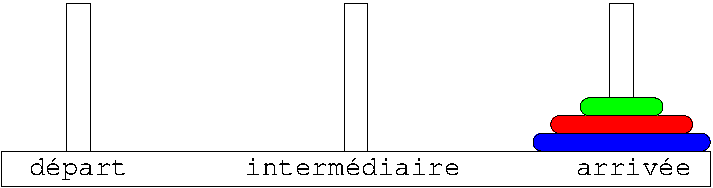
\includegraphics[width=8cm]{hanoi1.pdf}}

\end{frame}
\note{
\begin{rem}[Tours de Hanoï]
Les « tours de Hanoï » est un jeu imaginé par le mathématicien 
français Édouard Lucas (1842-1891). Il 
consiste à déplacer $n$ disques de diamètres différents d'une 
tour de « départ » à une tour d'« arrivée » en passant par une 
tour « intermédiaire » et ceci en un minimum de coups, 
tout en respectant les règles suivantes :
\begin{itemize}
\item on ne peut déplacer qu'un disque à la fois,
\item on ne peut placer un disque que sur un autre disque 
	plus grand que lui ou sur une tour vide.
\end{itemize}
\end{rem}
\null\vfill

\begin{td}[Tours de Hanoï {\em à la main}]
Résoudre {\em à la main} le problème des tours de Hanoï à $n$ disques successivement 
pour $n=1$, $n=2$, $n=3$ et $n=4$.
\end{td}
}
%------------------------------------------


%------------------------------------------
\begin{frame}
\frametitle{\uppercase{Appels récursifs}}
\framesubtitle{\uppercase{Tours de Hanoï}}
%------------------------------------------
\begin{columns}[T]
\column{6cm}
\begin{py}{6cm}\tt
def hanoi(n,gauche,milieu,droit):\\
\mbox{}\ \ \ \ assert type(n) is int\\
\mbox{}\ \ \ \ assert n >= 0\\
\mbox{}\ \ \ \ if n > 0:\\
\mbox{}\ \ \ \ \ \ \ \ \alert{hanoi(n-1,gauche,droit,milieu)}\\
\mbox{}\ \ \ \ \ \ \ \ deplacer(n,gauche,droit)\\
\mbox{}\ \ \ \ \ \ \ \ \alert{hanoi(n-1,milieu,droit,gauche)}\\
\mbox{}\ \ \ \ return\\
\mbox{}\\
%\pause
def deplacer(n,gauche,droit):\\
\mbox{}\ \ \ \ print('déplacer disque', n,\\
\mbox{}\ \ \ \ \ \ \ \ \ \ 'de la tour', gauche, \\
\mbox{}\ \ \ \ \ \ \ \ \ \ 'à la tour', droit)\\
\mbox{}\ \ \ \ return
\end{py}
%\pause
\column{5cm}
\begin{py}{5cm}\tt
\alert{>{>}> hanoi(3,'d','i','a')}\\
\mbox{}
\end{py}

\centerline{\includegraphics[width=3.9cm]{recursivite2.pdf}}
\end{columns}
\end{frame}
\note{
\null\vfill

\begin{rem}[Récursivité en arbre : {\tt hanoi}]
L'exécution d'un appel à la procédure {\tt hanoi} s'apparente ici encore
à un processus récursif en arbre : les 7 déplacements effectués lors
de l'appel {\tt hanoi(3,'d','i','a')} sont numérotés dans leur ordre d'apparition
sur la figure (les appels à la fonction {\tt hanoi}
pour {\tt n = 0} ne font rien). 

Mais toutes les fonctions récursives ne
conduisent pas nécessairement à un processus récursif en arbre 
comme l'exemple de la fonction {\tt factorielle} le montrera.
\end{rem}
}
%------------------------------------------


%------------------------------------------
\begin{frame}
\frametitle{\uppercase{Appels récursifs}}
\framesubtitle{\uppercase{Courbes fractales}}
%------------------------------------------
\begin{columns}
\column{7.25cm}
$$\includegraphics[width=7cm,angle=-90]{vonkock.jpg}$$
%\pause

\column{5cm}
\begin{py}{4.9cm}\tt
def kock(n,d):\\
\mbox{}\ \ \ \ if n == 0: forward(d)\\
\mbox{}\ \ \ \ else:\\
\mbox{}\ \ \ \ \ \ \ \ kock(n-1,d/3.)\\
\mbox{}\ \ \ \ \ \ \ \ left(60)\\
\mbox{}\ \ \ \ \ \ \ \ kock(n-1,d/3.)\\
\mbox{}\ \ \ \ \ \ \ \ right(120)\\
\mbox{}\ \ \ \ \ \ \ \ kock(n-1,d/3.)\\
\mbox{}\ \ \ \ \ \ \ \ left(60)\\
\mbox{}\ \ \ \ \ \ \ \ kock(n-1,d/3.)\\
\mbox{}\ \ \ \ return
\end{py}
\end{columns}

\end{frame}
\note{
\begin{rem}[Courbes de Koch]
La courbe de von Koch \index{{{\sc Von Koch}}} est l'une des premières courbes 
fractales à avoir été décrite par le mathématicien suédois Helge von Koch (1870-1924).
On peut la créer à partir d'un segment de droite, en modifiant récursivement 
chaque segment de droite de la façon suivante :
\begin{enumerate}
\item on divise le segment de droite en trois segments de longueurs égales,
\item on construit un triangle équilatéral ayant pour base le segment médian 
	de la première étape,
\item on supprime le segment de droite qui était la base du triangle 
	de la deuxième étape.
\end{enumerate}
\end{rem}
\null\vfill

\begin{td}[Flocons de Koch]
Définir une fonction qui dessine les flocons de Koch heptagonaux ci-dessous.
Généraliser à des polygones réguliers quelconques (triangle équilatéral, carré, pentagone régulier\ldots).
$$\includegraphics[width=4.5cm]{flocon2.jpg}$$
\end{td}
}
%------------------------------------------

%------------------------------------------
\begin{frame}
\frametitle{\uppercase{Appels récursifs}}
\framesubtitle{\uppercase{Fonction factorielle}}
%------------------------------------------
$$\left\{\begin{array}{l@{\ =\ }ll}
0! & 1 & \\
n! & n\cdot (n-1)! & \forall n \in N^*
\end{array}\right.$$
\vspace*{1cm}

%\pause
\begin{columns}[T]
\column{5.25cm}
\begin{py}{5.25cm}
{\bf Version itérative :}\\\tt
def factorielle(n):\\
\mbox{}\ \ \ \ u = 1\\
\mbox{}\ \ \ \ for i in range(2,n+1):\\
\mbox{}\ \ \ \ \ \ \ \ u = u * i\\
\mbox{}\ \ \ \ return u
\end{py}
%\pause
\column{5.25cm}
\begin{py}{5.25cm}
{\bf Version récursive :}\\\tt
def factorielle(n):\\
\mbox{}\ \ \ \ u = 1\\
\mbox{}\ \ \ \ if n > 1:\\
\mbox{}\ \ \ \ \ \ \ \ \alert{u = n * factorielle(n-1)}\\
\mbox{}\ \ \ \ return u
\end{py}
\end{columns}

\end{frame}
\note{
\null\vfill

\begin{td}[Pgcd et ppcm de 2 entiers]
\begin{enumerate}
\item Définir une fonction récursive qui calcule le plus grand 
	commun diviseur $d$ de 2 entiers $a$ et $b$ : \\
	$\rm{pgcd}(a,b) = \rm{pgcd}(b,a \bmod b) = \ldots 
	\ldots = \rm{pgcd}(d,0) = d$.
\item En déduire une fonction qui calcule le plus petit commun multiple $m$ de 2 entiers $a$ et $b$.
\end{enumerate}
\end{td}
\begin{td}[Somme arithmétique]
\begin{enumerate}
\item Définir une fonction récursive qui calcule la somme des 
	$n$ premiers nombres entiers.
	$$s = \sum^{n}_{k=0}k = \frac{n(n+1)}{2}$$
\item Comparer la complexité de cette version avec les versions
	constante et itérative.
\end{enumerate}
\end{td}
}
%------------------------------------------

%------------------------------------------
\begin{frame}
\frametitle{\uppercase{Appels récursifs}}
\framesubtitle{\uppercase{Fonction factorielle}}
%------------------------------------------
$$\begin{minipage}{8cm}\tt
\alert{>>> factorielle(5)}\\%\pause
\mbox{}\ \ \ \ \ \ \ \ (5*factorielle(4))\\%\pause
\mbox{}\ \ \ \ \ \ \ \ (5*(4*factorielle(3)))\\%\pause
\mbox{}\ \ \ \ \ \ \ \ (5*(4*(3*factorielle(2))))\\%\pause
\mbox{}\ \ \ \ \ \ \ \ (5*(4*(3*(2*factorielle(1)))))\\%\pause
\mbox{}\ \ \ \ \ \ \ \ (5*(4*(3*(2*1))))\\%\pause
\mbox{}\ \ \ \ \ \ \ \ (5*(4*(3*2)))\\%\pause
\mbox{}\ \ \ \ \ \ \ \ (5*(4*6))\\%\pause
\mbox{}\ \ \ \ \ \ \ \ (5*24)\\%\pause
\alert{120}
\end{minipage}$$

\end{frame}
\note{
\null\vfill

\begin{rem}[Récursivité linéaire : {\tt factorielle}]
La version récursive est la traduction directe
de la formulation mathématique. Dans la version récursive,
le processus nécessite que l'interpréteur garde une trace des multiplications
à réaliser plus tard. Le processus croît
puis décroît : la croissance se produit lorsque le processus construit une chaîne
d'opérations différées (ici, une chaîne de multiplications différées) et 
la décroissance intervient lorsqu'on peut évaluer les multiplications.

Ainsi, la quantité d'information qu'il faut mémoriser pour effectuer plus tard
les opérations différées croît linéairement avec $n$ : on parle de processus
récursif linéaire. 
\end{rem}
}
%------------------------------------------

%------------------------------------------
\begin{frame}
\frametitle{\uppercase{Appels récursifs}}
\framesubtitle{\uppercase{Fonction factorielle}}
%------------------------------------------
\begin{columns}[T]
\column{6.4cm}
\begin{py}{6.4cm}\tt
def factorielle(n):\\
\mbox{}\ \ \ \ u = factIter(n,1,1)\\
\mbox{}\ \ \ \ return u\\
\mbox{}\\%\pause
def factIter(n,i,fact):\\
\mbox{}\ \ \ \ u = fact\\
\mbox{}\ \ \ \ if i < n:\\
\mbox{}\ \ \ \ \ \ \ \ u = factIter(n,i+1,fact*(i+1))\\
\mbox{}\ \ \ \ return u
\end{py}
%\pause
\column{4.5cm}
\begin{py}{4.5cm}\tt
\alert{>{>}> factorielle(5)}\\%\pause
\mbox{}\ \ \ \ \ \ \ \ (factIter(5,1,1))\\%\pause
\mbox{}\ \ \ \ \ \ \ \ (factIter(5,2,2))\\%\pause
\mbox{}\ \ \ \ \ \ \ \ (factIter(5,3,6))\\%\pause
\mbox{}\ \ \ \ \ \ \ \ (factIter(5,4,24))\\%\pause
\mbox{}\ \ \ \ \ \ \ \ (factIter(5,5,120))\\%\pause
\alert{120}
\end{py}
\end{columns}

\end{frame}
\note{
{\bf Définitions}\begin{description}
\item[récursivité terminale]
Un appel récursif terminal est un appel récursif dont le résultat est celui 
retourné par la fonction.
\item[récursivité non terminale]
Un appel récursif non terminal est un appel récursif dont le résultat 
n'est pas celui retourné par la fonction.
\end{description}
\null\vfill

\begin{rem}
La nouvelle fonction {\tt factorielle} appelle une fonction
auxiliaire {\tt factIter} dont la définition est syntaxiquement récursive
({\tt factIter} s'appelle elle-même). Cette fonction à 3 arguments : l'entier {\tt n} 
dont il faut calculer la factorielle, un compteur {\tt i} initialisé à {\tt 1}
au premier appel de {\tt factIter} par {\tt factorielle} et incrémenté à chaque
nouvel appel, et un nombre {\tt fact} initialisé à {\tt 1} et multiplié
par la nouvelle valeur du compteur à chaque nouvel appel. 

Le déroulement
d'un appel à {\tt factIter} montre qu'ainsi, à chaque étape, la relation
{\tt (i! == fact)} est toujours vérifiée. La fonction {\tt factIter}
arrête de s'appeler elle-même lorsque {\tt (i == n)} et on a alors 
{\tt (fact == i! == n!)} qui est la valeur recherchée. 

Ainsi, à chaque étape,
nous n'avons besoin que des valeurs courantes du compteur {\tt i} 
et du produit {\tt fact},
exactement comme dans la version itérative de la fonction {\tt factorielle} :
il n'y a plus de chaîne d'opérations différées comme dans la version récursive
de {\tt factorielle}. Le processus mis en jeu ici est un processus itératif, 
bien que la définition de {\tt factIter} soit récursive.
\end{rem}
}


%------------------------------------------
\begin{frame}<presentation>
\frametitle{\uppercase{Appels récursifs}}
\framesubtitle{\uppercase{récursivité terminale $\rightarrow$ boucle}}
%------------------------------------------
\begin{columns}[T]
\column{4cm}
\begin{py}{4cm}\tt
def f(x):\\
\mbox{}\ \ \ \ if cond: arret\\
\mbox{}\ \ \ \ else:\\
\mbox{}\ \ \ \ \ \ \ \ instructions\\
\mbox{}\ \ \ \ \ \ \ \ f(g(x))\\
\mbox{}\ \ \ \ return
\end{py}
%\pause

$$\alert{\Downarrow}$$

\begin{py}{4cm}\tt
def f(x):\\
\mbox{}\ \ \ \ while not cond: \\
\mbox{}\ \ \ \ \ \ \ \ instructions\\
\mbox{}\ \ \ \ \ \ \ \ x = g(x)\\
\mbox{}\ \ \ \ arret\\
\mbox{}\ \ \ \ return
\end{py}
%\pause

\column{6.5cm}
\begin{py}{6.5cm}\tt
def factIter(n,i,fact):\\
\mbox{}\ \ \ \ if i >= n: u = fact\\
\mbox{}\ \ \ \ else:\\
\mbox{}\ \ \ \ \ \ \ \ pass\\
\mbox{}\ \ \ \ \ \ \ \ u = factIter(n,i+1,fact*(i+1))\\
\mbox{}\ \ \ \ return u
\end{py}
%\pause

$$\alert{\Downarrow}$$

\begin{py}{6.5cm}\tt
def factIter(n,i,fact):\\
\mbox{}\ \ \ \ while i < n:\\
\mbox{}\ \ \ \ \ \ \ \ pass\\
\mbox{}\ \ \ \ \ \ \ \ n,i,fact = n,i+1,fact*(i+1)\\
\mbox{}\ \ \ \ u = fact\\
\mbox{}\ \ \ \ return u
\end{py}
\end{columns}

\end{frame}
\note{
\begin{rem}[Elimination de la récursivité]
La méthode précédente ne s'applique qu'à la récursivité terminale.

Une méthode générale existe pour transformer une fonction récursive
quelconque en une fonction itérative équivalente. En particulier,
elle est mise en \oe uvre dans les compilateurs car le langage machine 
n'admet pas la récursivité. Cette méthode générale fait appel à la notion 
de pile pour sauvegarder
le contexte des appels récursifs. 
\end{rem}
\null\vfill

\begin{td}[Pgcd]
Transformer la fonction récursive ci-dessous en une fonction itérative.
\vspace*{3mm}

\begin{minipage}{7cm}\tt
def pgcd(a,b):\\
\mbox{}\ \ \ \ if b == 0: d = a\\
\mbox{}\ \ \ \ else: d = pgcd(b,a\%b)\\
\mbox{}\ \ \ \ return d
\end{minipage}
\end{td}
}
%------------------------------------------


%-------------------------------------------------------------------------
\end{document}
%-------------------------------------------------------------------------
